%=============================================================================
% Chapter 5: Strings in C++
%=============================================================================
\chapter{Strings in C++}
\label{ch:strings}

%-----------------------------------------------------------------------------
\section{Introduction to Strings}
\label{sec:strings-intro}
%-----------------------------------------------------------------------------

\begin{definitionbox}{C-Style Strings}
In C++ strings of characters are implemented as an array of characters
with a \textbf{null terminator} \texttt{'\textbackslash 0'}.  The null
character marks the end of the string so that library functions know where
the string data stops.
\end{definitionbox}

\noindent
The general form for declaring a character string is:

\begin{cppcode}
char String_name[size];
\end{cppcode}

\noindent
where \texttt{size} specifies the maximum number of characters the array
can hold, \emph{including} the null terminator.

\subsection{Initialising Strings}

A string can be initialised at declaration time in several ways:

\begin{cppcode}
char name[11] = "Mazin Alaa";   // size must include '\0'
char str[]    = "ABCD";         // compiler sets size = 5
\end{cppcode}

\begin{warningbox}{Size Must Include the Null Terminator}
When you specify the size explicitly, remember to count the
\texttt{'\textbackslash 0'} character.  For example,
\texttt{"Mazin Alaa"} has 10 visible characters, so the array must be
at least \texttt{[11]}.
\end{warningbox}

\subsection{Character-by-Character Storage}

When the compiler stores \texttt{str[] = "ABCD"}, the memory layout is
as follows:

\begin{center}
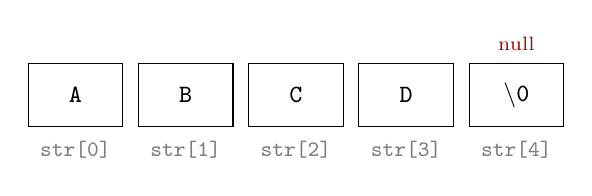
\begin{tikzpicture}[
    cell/.style={draw, minimum width=1.2cm, minimum height=0.8cm,
                 font=\ttfamily\small},
    label/.style={font=\footnotesize\ttfamily, text=gray}
]
  \foreach \c/\i in {A/0, B/1, C/2, D/3, \textbackslash 0/4} {
    \node[cell] (c\i) at (\i*1.4, 0) {\c};
    \node[label] at (\i*1.4, -0.7) {str[\i]};
  }
  \node[font=\scriptsize, text=red!70!black] at (4*1.4, 0.65)
       {null};
\end{tikzpicture}
\end{center}

\begin{importantbox}{The Null Terminator}
The character \texttt{'\textbackslash 0'} (ASCII value 0) is
automatically appended by the compiler when you use a string literal.
Without it, functions such as \texttt{cout}, \texttt{strlen}, and
\texttt{strcpy} will read past the intended boundary, causing
undefined behaviour.
\end{importantbox}

%-----------------------------------------------------------------------------
\section{Reading, Writing, and Processing Strings}
\label{sec:strings-rw}
%-----------------------------------------------------------------------------

\subsection{Example 1 --- Printing a String}

The following program prints an entire string and then prints it
character by character using a loop:

\begin{cppcode}
#include <iostream>
using namespace std;

int main() {
    char str[] = "Hello, World!";

    // Print the whole string at once
    cout << "Full string: " << str << endl;

    // Print character by character
    cout << "Char by char: ";
    for (int i = 0; str[i] != '\0'; i++) {
        cout << str[i];
    }
    cout << endl;

    return 0;
}
\end{cppcode}

\noindent
\textbf{Sample run:}
\begin{verbatim}
Full string: Hello, World!
Char by char: Hello, World!
\end{verbatim}

\begin{conceptbox}{Iterating Over a C-String}
The idiomatic way to walk through a C-string is to loop while
\texttt{str[i] != '\textbackslash 0'}.  This works because every
properly formed C-string is guaranteed to end with the null character.
\end{conceptbox}

\subsection{Example 2 --- Converting Lowercase to Uppercase}

The library function \texttt{toupper()} (declared in
\texttt{<cctype>}) converts a single lowercase letter to its uppercase
equivalent.  Non-lowercase characters are returned unchanged.

\begin{cppcode}
#include <iostream>
#include <cctype>
using namespace std;

int main() {
    char str[50];

    cout << "Enter a string: ";
    cin.getline(str, 50);

    for (int i = 0; str[i] != '\0'; i++) {
        str[i] = toupper(str[i]);
    }

    cout << "Uppercase: " << str << endl;

    return 0;
}
\end{cppcode}

\noindent
\textbf{Sample run:}
\begin{verbatim}
Enter a string: Hello World
Uppercase: HELLO WORLD
\end{verbatim}

%-----------------------------------------------------------------------------
\section{String I/O Functions}
\label{sec:strings-io}
%-----------------------------------------------------------------------------

\begin{infobox}{Useful String I/O Functions}
\begin{tabular}{@{}l l@{}}
\texttt{cin.getline(str, n);} & Read up to \texttt{n-1} characters
    (including spaces) into \texttt{str}. \\[4pt]
\texttt{cin.get(ch);}         & Read a single character (including
    whitespace) into \texttt{ch}. \\[4pt]
\texttt{cin.ignore(n, delim);} & Discard up to \texttt{n} characters
    or until \texttt{delim} is found. \\[4pt]
\texttt{cin.putback(ch);}     & Push character \texttt{ch} back into
    the input buffer. \\[4pt]
\texttt{cout.put(ch);}        & Write a single character to standard
    output. \\
\end{tabular}
\end{infobox}

\begin{cppcode}
#include <iostream>
using namespace std;

int main() {
    char line[80], ch;

    cout << "Enter a line: ";
    cin.getline(line, 80);       // reads full line with spaces
    cout << "You entered: " << line << endl;

    cout << "Enter a character: ";
    cin.get(ch);                 // reads one character
    cout << "Character: ";
    cout.put(ch);                // writes one character
    cout << endl;

    cin.ignore(80, '\n');        // flush remaining input

    return 0;
}
\end{cppcode}

\noindent
\textbf{Sample run:}
\begin{verbatim}
Enter a line: Programming is fun
You entered: Programming is fun
Enter a character: X
Character: X
\end{verbatim}

\begin{warningbox}{\texttt{cin >>} vs.\ \texttt{cin.getline()}}
The extraction operator \texttt{>>} stops reading at the first
whitespace character, so it cannot read a full sentence.  Use
\texttt{cin.getline()} when you need to capture an entire line
including spaces.
\end{warningbox}

%-----------------------------------------------------------------------------
\section{String Library Functions (\texttt{string.h})}
\label{sec:string-lib}
%-----------------------------------------------------------------------------

The header \texttt{<cstring>} (or the older \texttt{<string.h>})
provides a rich set of functions for manipulating C-style strings.
Table~\ref{tab:string-funcs} summarises the most commonly used ones.

\begin{table}[htbp]
\centering
\caption{Common \texttt{<cstring>} library functions.}
\label{tab:string-funcs}
\renewcommand{\arraystretch}{1.4}
\begin{tabular}{@{} l p{4.8cm} p{5.5cm} @{}}
\toprule
\textbf{Function} & \textbf{Description} & \textbf{Example} \\
\midrule
\texttt{strlen(s)} &
    Returns the number of characters in \texttt{s}, \emph{excluding}
    the null terminator. &
    \texttt{char a[]="abcd";}\newline
    \texttt{cout << strlen(a);}\newline
    \textit{Output:} \texttt{4} \\
\addlinespace
\texttt{strcpy(dest, src)} &
    Copies the string \texttt{src} (including \texttt{'\textbackslash 0'})
    into \texttt{dest}. &
    \texttt{char a[]="abcd", b[10];}\newline
    \texttt{strcpy(b, a);}\newline
    \textit{b is now} \texttt{"abcd"} \\
\addlinespace
\texttt{strcat(s1, s2)} &
    Appends a copy of \texttt{s2} to the end of \texttt{s1}.
    \texttt{s1} must have enough room. &
    \texttt{char a[20]="abcd";}\newline
    \texttt{char b[]="1234";}\newline
    \texttt{strcat(a, b);}\newline
    \textit{a is now} \texttt{"abcd1234"} \\
\addlinespace
\texttt{strcmp(s1, s2)} &
    Compares two strings lexicographically.\newline
    Returns \texttt{0} if equal, a positive value if
    \texttt{s1 > s2}, a negative value if \texttt{s1 < s2}. &
    \texttt{strcmp("abc","abc");} $\rightarrow$ \texttt{0}\newline
    \texttt{strcmp("b","a");}\ \ $\rightarrow$ \texttt{+}\newline
    \texttt{strcmp("a","b");}\ \ $\rightarrow$ \texttt{-} \\
\bottomrule
\end{tabular}
\end{table}

\begin{cppcode}
#include <iostream>
#include <cstring>
using namespace std;

int main() {
    char s1[30] = "Hello";
    char s2[]   = " World";

    cout << "Length of s1: " << strlen(s1) << endl;   // 5

    strcat(s1, s2);
    cout << "After strcat: " << s1 << endl;           // Hello World

    char s3[30];
    strcpy(s3, s1);
    cout << "Copied s3:    " << s3 << endl;           // Hello World

    if (strcmp(s1, s3) == 0)
        cout << "s1 and s3 are equal." << endl;

    return 0;
}
\end{cppcode}

\noindent
\textbf{Sample run:}
\begin{verbatim}
Length of s1: 5
After strcat: Hello World
Copied s3:    Hello World
s1 and s3 are equal.
\end{verbatim}

\begin{warningbox}{Buffer Overflow with C-Strings}
C-style string functions such as \texttt{strcpy()} and \texttt{strcat()}
do \emph{not} check whether the destination array is large enough.
Writing past the end of the array causes a \textbf{buffer overflow},
which can corrupt other variables, crash the program, or create
security vulnerabilities.  Always ensure the destination has
enough room, including the null terminator.
\end{warningbox}

%-----------------------------------------------------------------------------
\section{\texttt{stdlib} Library Functions}
\label{sec:stdlib-funcs}
%-----------------------------------------------------------------------------

The header \texttt{<cstdlib>} provides functions for converting between
strings and numeric types.  Table~\ref{tab:stdlib-funcs} lists the most
important ones.

\begin{table}[htbp]
\centering
\caption{Common \texttt{<cstdlib>} conversion functions.}
\label{tab:stdlib-funcs}
\renewcommand{\arraystretch}{1.4}
\begin{tabular}{@{} l p{4.5cm} p{5.8cm} @{}}
\toprule
\textbf{Function} & \textbf{Description} & \textbf{Example} \\
\midrule
\texttt{atoi(s)} &
    Converts the string \texttt{s} to an \texttt{int}. &
    \texttt{char a[]="1234";}\newline
    \texttt{int i = atoi(a);}\newline
    \textit{i is now} \texttt{1234} \\
\addlinespace
\texttt{atof(s)} &
    Converts the string \texttt{s} to a \texttt{double}. &
    \texttt{char a[]="12.34";}\newline
    \texttt{double f = atof(a);}\newline
    \textit{f is now} \texttt{12.34} \\
\addlinespace
\texttt{itoa(i, s, base)} &
    Converts the integer \texttt{i} to a string stored in \texttt{s}
    using the specified \texttt{base} (e.g.\ 10 for decimal). &
    \texttt{int i = 1234;}\newline
    \texttt{char a[10];}\newline
    \texttt{itoa(i, a, 10);}\newline
    \textit{a is now} \texttt{"1234"} \\
\bottomrule
\end{tabular}
\end{table}

\begin{warningbox}{\texttt{itoa} is Non-Standard}
The function \texttt{itoa()} is not part of the C++ standard; it is a
compiler extension available in some implementations (e.g.\ older
Borland and MSVC compilers).  For portable code, prefer
\texttt{sprintf()} or \texttt{std::to\_string()} (C++11).
\end{warningbox}

\begin{cppcode}
#include <iostream>
#include <cstdlib>
using namespace std;

int main() {
    // String to integer
    char num_str[] = "2048";
    int num = atoi(num_str);
    cout << "Integer: " << num << endl;        // 2048

    // String to floating point
    char flt_str[] = "3.14159";
    double pi = atof(flt_str);
    cout << "Double:  " << pi << endl;         // 3.14159

    // Integer to string (non-standard)
    // int val = 255;
    // char buf[20];
    // itoa(val, buf, 10);
    // cout << "String:  " << buf << endl;     // 255

    return 0;
}
\end{cppcode}

\noindent
\textbf{Sample run:}
\begin{verbatim}
Integer: 2048
Double:  3.14159
\end{verbatim}

\begin{warningbox}{Missing Null Terminator}
If you build a string character by character (e.g.\ inside a loop),
you \emph{must} append \texttt{'\textbackslash 0'} manually after the
last character.  Forgetting it means that every function expecting a
C-string will read beyond the intended data, leading to garbage output
or undefined behaviour.
\end{warningbox}

\begin{conceptbox}{C-Strings vs.\ \texttt{std::string}}
Modern C++ provides the \texttt{std::string} class (from
\texttt{<string>}) which handles memory management automatically and
supports intuitive operators such as \texttt{+} for concatenation and
\texttt{==} for comparison.  However, understanding C-style strings is
essential because they appear in legacy code, system-level
programming, and many library interfaces.
\end{conceptbox}
